\section{Br/As 与其它核区的反射---手征问题}\label{sec:4-5}

在奇奇核与奇 $A$ 核的高自旋谱学中，当实验能级纲图上同时呈现出两对具有相近能量序列的正负宇称能带、且正负宇称带之间观测到相互交织的电偶极 $E1$ 连接跃迁时，一个引人瞩目的科学问题随之产生：这些在实验室系中呈现相近能级间隔的状态，是否如早期文献所探讨的那样，属于内禀手征对称性与空间反射对称性同时发生自发破缺所形成的“手征---宇称四重简并带（Chiral-Reflection Quartet, CPQ）”？

在理想的理论几何图像中，若原子核具备稳定的三轴非对称核芯（使四极内禀密度不再轴对称）并同时具备非平面的三维角动量几何（打破手征对称性），同时具备稳定的梨形八极形变（打破空间反演对称性），在固定有向体轴且确有相关定域构型的理想图像中，可用手征左右与八极朝向标记四个内禀构型；是否形成四个独立投影低能态仍须检验。必须明确指出：三轴形变本身仅打破轴对称性，并不自动导致手征对称性破缺；手征对称性自发破缺严格要求价质子、价中子与三轴核芯集体转动角动量矢量在空间构成非平面的三维取向结构。此外，第\ref{sec:2-5}节建立的量子投影恢复原理以及第\ref{sec:3-5}节对手征几何的微观解构明确指出：内禀平均场波函数的对称性破缺并不等价于实验室体系中四条能带的严格简并。特别是在 $A \approx 80$ 过渡核区中，单粒子自由度、三轴柔顺性与微观形状涨落紧密交织。本节以山东大学刘晨等人（2016年）关于 $^{78}\mathrm{Br}$ 的实验工作与肖骁等人（2019/2022年）关于 $^{74}\mathrm{As}$ 的实验工作为主线，从第一手测量链与实际跃迁网络出发，系统辨析该核区的数据现状与理论解释，阐明当前实验数据尚不足以确立来自同一相关内禀构型空间的静态手征---宇称四重带，厘清实验室好宇称态与内禀反射不对称的本质区别，解离内禀电偶极矩 $D_0$ 的模型依赖性，并给出该前沿方向上可证伪的研究检验路径~\cite{liu-2016-octupole-correlations-multiple-chiral-doublet-bands-78br,liu-chen-2016-78br-chirality-reflection-symmetry-thesis,xiao-2022-chirality-octupole-correlations-74as,xiao-xiao-2019-high-spin-74as-thesis,butler-1996-octupole-shapes,wang-2019-rat-prm-78br-octupole-correlations}。

\subsection{可追溯的能带结构与实际测量载荷}\label{sec:4-5-1}

为了确保学术讨论完全建立在经过严格实验检验的客观事实之上，表~\ref{tab:4-5-bands-summary}汇总了 $^{78}\mathrm{Br}$ 与 $^{74}\mathrm{As}$ 在第一手在束实验中实际观测到的能带编号、自旋宇称范围、微观组态指派以及直接测得的特征跃迁参量。

\begin{table}[!htbp]
\centering
\footnotesize
\caption{$^{78}\mathrm{Br}$ 与 $^{74}\mathrm{As}$ 中相关能带的观测自旋范围、组态指派与实验测量载荷汇总（严格依据刘晨 2016 博士论文与 PRL 2016、肖骁 2019 硕士论文与 PRC 2022 原件核对）。}\label{tab:4-5-bands-summary}
\begin{tabularx}{\textwidth}{p{2.0cm}p{1.6cm}p{1.9cm}p{3.0cm}>{\raggedright\arraybackslash}X}
\hline\hline
核素与反应条件 & 能带标识 & 自旋宇称范围 & 微观组态指派 & 实测跃迁网络与客观测量边界 \\
\hline
$^{78}\mathrm{Br}$ & Band 1 ($\pi=+$) & $7^+$ 至 $(20^+)$（图1） & $\pi g_{9/2} \otimes \nu g_{9/2}$ & 带内 $E2$ 级联；通过 $\Delta I=1$ 跃迁接收 Band 2 馈送；由 8 条 $E1$ 跃迁与 Band 3 互连；所引工作未给相关带的绝对寿命 \\
\shortstack[l]{$^{70}\mathrm{Zn}$\\$(^{12}\mathrm{C}, p3n)$} & Band 2 ($\pi=+$) & $9^+$ 至 $13^+$（图1） & $\pi g_{9/2} \otimes \nu g_{9/2}$ & 测得 ADO 比值与线偏振度；与 Band 1 构成手征候选双带；在当前探测灵敏度下未测得连接至负宇称带的 $E1$ 跃迁 \\
60, 65 MeV & Band 3 ($\pi=-$) & $6^-$ 至 $(19^-)$（图1） & $\pi f_{5/2}(p_{3/2}) \otimes \nu g_{9/2}$ & 带内 $E2$ 级联；测得带间分支比 $B(E1)/B(E2)$；由 8 条 $E1$ 跃迁连接至 Band 1；所引工作未给相关带的绝对寿命 \\
iThemba AFRODITE & Band 4 ($\pi=-$) & $6^-$ 至 $(14^-)$（2016图1） & $\pi f_{5/2}(p_{3/2}) \otimes \nu g_{9/2}$ & 经 $404.3\ \mathrm{keV}$ 跃迁退激至 Band 3；与 Band 3 构成手征候选；在当前探测限度下未测得跨宇称 $E1$ 跃迁 \\
\hline
$^{74}\mathrm{As}$ & Band 1 ($\pi=+$) & $6^+$ 至 $(16^+)$（2022图1） & $\pi g_{9/2} \otimes \nu g_{9/2}$ & 带内 $E2$ 级联；与 Band 2 发生 $\Delta I=1$ 混合；由 3 条 $E1$ 跃迁接收 Band 3 馈送；所引工作未给相关带的绝对寿命 \\
\shortstack[l]{$^{74}\mathrm{Ge}$\\$(^4\mathrm{He}, 1p3n)$} & Band 2 ($\pi=+$) & $7^+$ 至 $(14^+)$（2022图1） & $\pi g_{9/2} \otimes \nu g_{9/2}$ & 测得 ADO 比值；$B(M1)/B(E2)$ 呈现奇偶交错；与 Band 1 构成手征双带；未见跨宇称连接 \\
58.6, 62.6 MeV & Band 3 ($\pi=-$) & 图1包含 $5^-,6^-$ 低端态，延伸至 $14^-$ & $\pi(f_{5/2}/p_{3/2}) \otimes \nu g_{9/2}$ & 带内 $E2$ 级联；由 $372.4, 919.4, 1293.4\ \mathrm{keV}$ 共 3 条 $E1$ 跃迁连接至 Band 1；所引工作未给相关带的绝对寿命 \\
iThemba AFRODITE & Band 4 ($\pi=-$) & 2019论文的负宇称序列；未与2022逐线映射 & 2019 学位报告候选带 & 2019 硕士论文纲图观测并指认（判定不满足手征判据，归为候选赝自旋伙伴带）；2022 期刊聚焦 1--3 带 \\
\hline\hline
\end{tabularx}
\end{table}

\textbf{实验谱系与数据源依赖性声明}：
必须明确澄清实验数据的谱系归属：刘晨博士论文中所比较的 $^{78}\mathrm{Br}$ 谱学部分与期刊 PRL 论文（Liu et al. 2016）同属在南非 iThemba LABS 利用 AFRODITE 高分辨锗探测阵列与 DIAMANT 带电粒子阵列开展的 $^{70}\mathrm{Zn}(^{12}\mathrm{C}, p3n)^{78}\mathrm{Br}$ 反应在束测量数据；肖骁硕士论文（2019年）与期刊 PRC 论文（Xiao et al. 2022）的相关测量同属在 iThemba LABS 利用 AFRODITE 阵列开展的 $^{74}\mathrm{Ge}(^4\mathrm{He}, 1p3n)^{74}\mathrm{As}$ 反应实验谱系。同一实验谱系的学位论文与期刊不能计作独立重复实验。不过，两版报告不必使用完全相同的事件选择或矩阵：2019论文约 $6.17\times10^9$ 与2022期刊约 $1.9\times10^9$ 的符合计数具有不同报告口径，尚没有共同门条件证明二者相同；刻度、子集与带号也应分别核对。

特别需要指出，对于 $^{74}\mathrm{As}$ 的负宇称能带结构，学术界存在不同的文献呈现版本：肖骁在其 2019 年硕士学位论文中构建了包含 thesis Band 4的完整能级纲图，并通过细致的 $S(I)$ 与惯量计算，明确论证了 Band 3 与 Band 4 并不满足严格的手征双重带判据，进而将其提出为可能的赝自旋伙伴带；而在 2022 年发表的正式期刊论文中，作者团队为了突出手征性与八极关联，集中报道了满足手征判据的正宇称双重带（Bands 1--2）以及与之具有强 $E1$ 跃迁连接的负宇称带（Band 3），期刊的负宇称Band 3与thesis Bands 3/4尚未完成唯一的逐线对应，不能仅按相同数字合并。因此，必须客观记录两个版本各自的学术侧重与原始报告，绝对不能武断宣称“Band 4 从未在实验中被观测到”。

\subsection{实际观测宇称连接网络拓扑}\label{sec:4-5-2}

根据原件测量数据绘制的能带连接网络如图~\ref{fig:4-5-network}所示。仔细审视实际跃迁网络的拓扑连接，有助于准确把握文献中关于“四重带”讨论的物理本质。

\begin{figure}[!htbp]
\centering
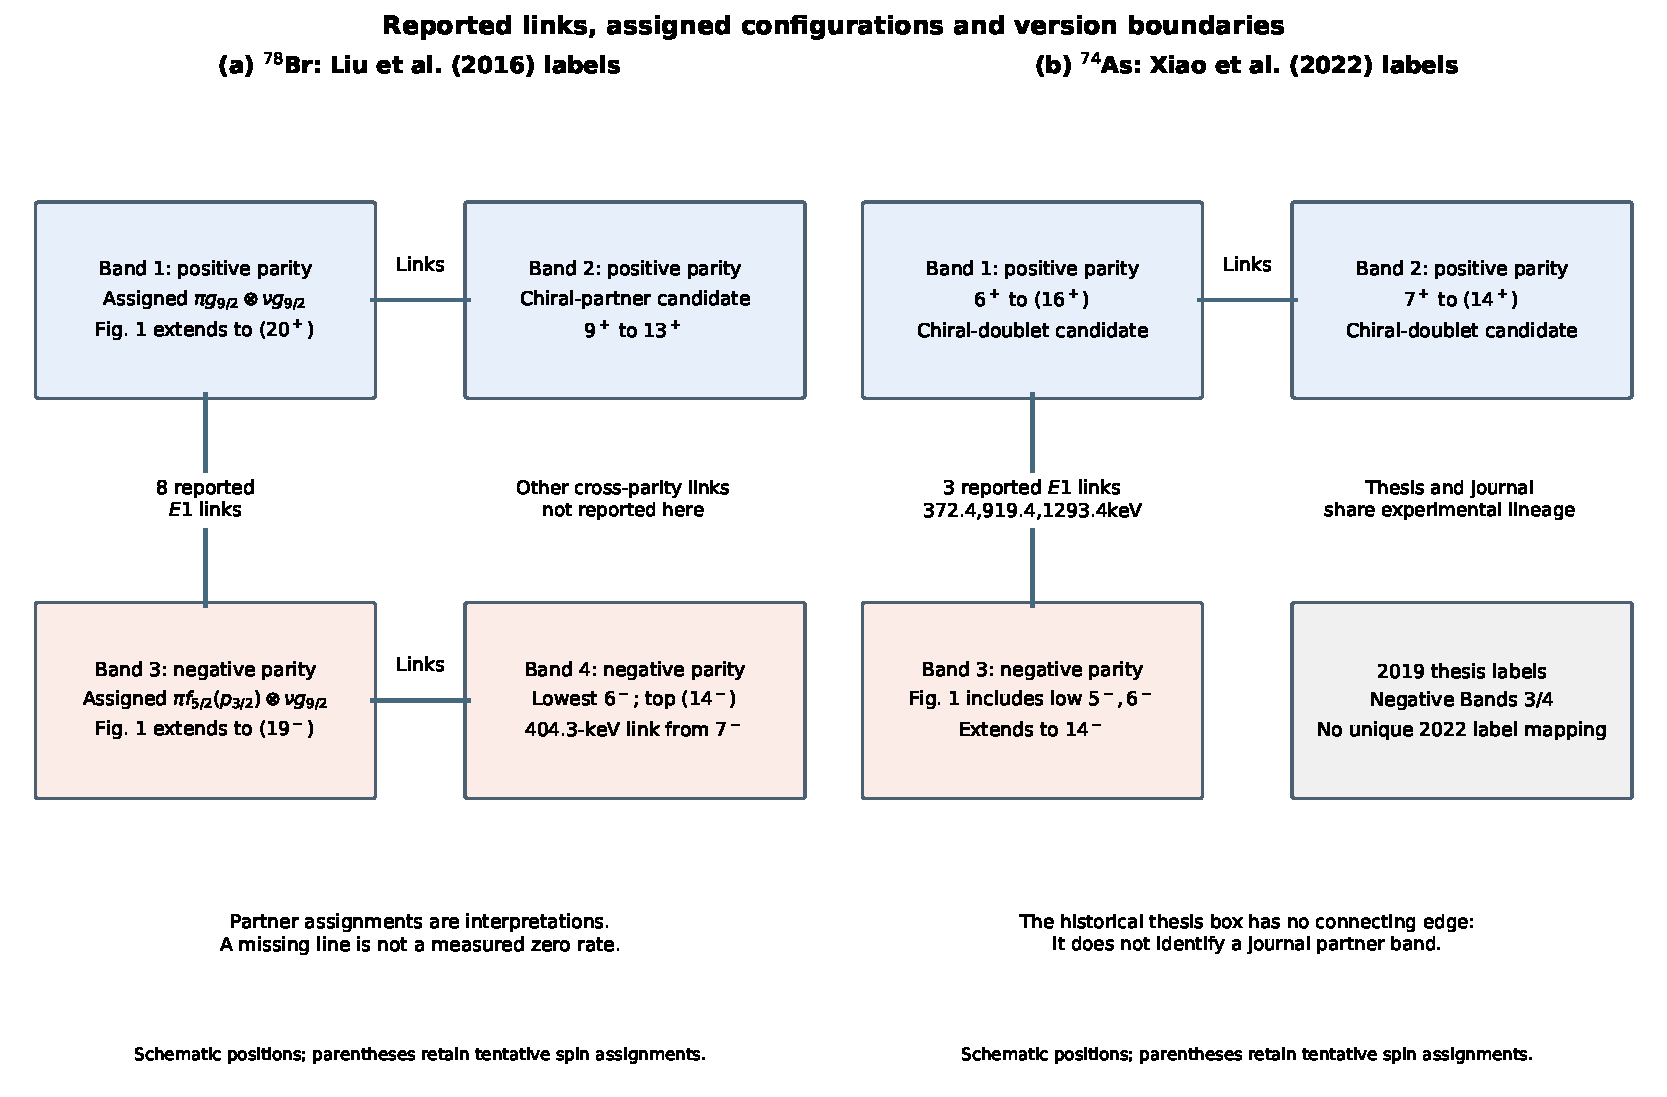
\includegraphics[width=0.88\textwidth]{Img/br-as-network-topology.pdf}
\caption[$^{78}\mathrm{Br}$ 与 $^{74}\mathrm{As}$ 实验中实际观测到的能带结构与跃迁连接网络拓扑示意图]{$^{78}\mathrm{Br}$ 与 $^{74}\mathrm{As}$ 实验中实际观测到的能带结构与跃迁连接网络拓扑示意图（依据 Liu et al. PRL 2016、刘晨 2016 博士论文、Xiao et al. PRC 2022 及肖骁 2019 硕士论文绘制；代码与数据来源见附录\ref{app:reproducible-inputs}）。(a) $^{78}\mathrm{Br}$ 中观测到的 4 条主带：正宇称带 Band 1, 2 与负宇称带 Band 3, 4 建立在不同的微观单粒子组态之上；8 条报告的 $E1$ 跃迁连接 Band 1 与 Band 3；图中连线只归纳带间联系，不表示一条光子跃迁具有双向发射率。其他连接未报告，所引资料未给统一数值上限；(b) $^{74}\mathrm{As}$ 中观测到的能带关联：正宇称双重带 Band 1, 2 与负宇称带 Band 3 通过 3 条实测 $E1$ 跃迁（$372.4, 919.4, 1293.4\ \mathrm{keV}$）互连；2019学位论文另有其负宇称Bands 3/4及候选赝自旋解释，未与2022负宇称带建立唯一逐线映射。}\label{fig:4-5-network}
\end{figure}

从图~\ref{fig:4-5-network}展示的真实网络拓扑中，可以得出两点明确的物理结论：
\begin{enumerate}
\item \textbf{$^{78}\mathrm{Br}$ 中的“多手征带伴随八极关联”与同构型静态四重带的区别}：
在 $^{78}\mathrm{Br}$ 中，正宇称能带（Band 1 与 Band 2）建立在 $\pi g_{9/2} \otimes \nu g_{9/2}$ 组态之上，由微观粒子--转子模型（TPRM）支持为一对正宇称手征双重带；而负宇称能带（Band 3 与 Band 4）建立在 $\pi f_{5/2}(p_{3/2}) \otimes \nu g_{9/2}$ 组态之上，被解释为另一对负宇称手征双重带。这两对能带在内禀组态上涉及不同的奇质子主导轨道占据。更关键的是，实验观测到的 8 条 $E1$ 连接跃迁局限在正宇称基带 Band 1 与负宇称带 Band 3 之间；在两个伴带 Band 2 与 Band 4 之间，以及 Band 2 与 Band 3、Band 1 与 Band 4 之间，在当前探测阵列统计限度内未测得明显的跨带 $E1$ 跃迁。需要指出，未见线需要结合效率、本底和统计选择才能量化为上限；所引资料未给出每条缺失连接的统一数值上限，不能据此置零；但作者将所见能带及模型比较解释为 $^{78}\mathrm{Br}$ 中基于所指派组态的多重手征双重带系统（Multiple Chiral Doublets, $M\chi D$）并伴随特定单侧能带间的八极关联，当前数据尚不足以确立在单一固定组态下由空间反射与手征同时破缺所构成的静态手征---宇称四重简并带。
\item \textbf{$^{74}\mathrm{As}$ 中缺乏闭合的四能带交织手征网络}：
在 $^{74}\mathrm{As}$ 中，2022 年期刊论文确立的强连接网络展现为 $2+1$ 的三能带结构：满足手征指纹的正宇称双重带（Band 1 与 Band 2）以及一条由 3 条 $E1$ 跃迁（$372.4, 919.4, 1293.4\ \mathrm{keV}$）连接的负宇称能带（Band 3）。即便在 2019 年学位论文包含了负宇称 Band 4 的原始纲图中，作者认为其负宇称Bands 3/4不满足所采用的手征判据，并保留赝自旋伙伴候选解释；这些是thesis自己的带号，不能把期刊E1网络倒赋给其中某一条。体系在现有实验精度下尚未展现出两对正负宇称手征双带对称交织构成的四重完全闭合网络。
\end{enumerate}

\subsection{理论概念桥梁：对称性、算符与几何误区}\label{sec:4-5-3}

面对上述实验拓扑，理论分析必须严格厘清不同离散对称性、量子力学算符以及表象之间的本质区别：

\subsubsection{实验室好宇称态与内禀反射不对称的区别}

在忽略弱相互作用宇称不守恒效应的核物理体系中，采用强相互作用与电磁相互作用哈密顿量 $\hat{H}$ 时，空间反演算符 $\hat{\mathcal{P}}$（$\mathbf{r} \to -\mathbf{r}$）与哈密顿量严格对易：
\begin{equation}\label{eq:4-5-parity-commute}
[\hat{H}, \hat{\mathcal{P}}] = 0.
\end{equation}
因此，在上述强与电磁哈密顿量下，体系的精确能量本征定态总可以选择为具有确定守恒空间宇称 $\pi = \pm 1$ 的好宇称态。文献中所讨论的“空间反射不对称性”，属于自洽平均场或内禀参考系近似下的物理图像。若微观平均场给出的能量极小态具备非零的内禀八极形变（$\beta_3 \neq 0$），则内禀波函数不具备确定的空间反射对称性：
\begin{equation}\label{eq:4-5-intrinsic-parity-breaking}
\hat{\mathcal{P}}\,|\Phi_{\mathrm{int}}(\beta_3)\rangle = |\Phi_{\mathrm{int}}(-\beta_3)\rangle \neq |\Phi_{\mathrm{int}}(\beta_3)\rangle .
\end{equation}
为了在实验室参考系中恢复精确守恒的角动量与空间宇称量子数，必须对内禀波函数执行严格的三维角动量与宇称联合投影。具有良好总角动量 $I$、实验室投影 $M$、确定宇称 $\pi$ 及能级指标 $\alpha$ 的物理态表示为：
\begin{equation}\label{eq:4-5-parity-projection}
|I M \pi; \alpha\rangle = \mathcal{N}_{I^\pi \alpha} \sum_K f_K^{I^\pi \alpha} \hat{P}_{MK}^I \left( \frac{1 + \pi \hat{\mathcal{P}}}{2} \right) |\Phi_{\mathrm{int}}\rangle ,
\end{equation}
这是所选有限投影试探空间中的构态方法，而非所有求解核态的方法都必须从该内禀态出发。其中 $\hat{P}_{MK}^I$ 为三维角动量投影算符，归一化因子 $\mathcal{N}_{I^\pi \alpha}$ 以及 $K$ 混合系数 $f_K^{I^\pi \alpha}$ 由该试探空间的角动量---宇称范数核、哈密顿核与广义本征问题确定；恢复量子数不保证变分空间已完备。单纯的宇称投影归一因子 $2(1 \pm \langle \Phi_{\mathrm{int}} | \hat{\mathcal{P}} | \Phi_{\mathrm{int}} \rangle)$ 仅适用于未投影角动量的一维情形，不能直接套用于包含三维欧拉角积分的复合投影态。

在一个存在两处反射相关定域构型的势阱模型中，量子混合可以使其宇称组合发生劈裂。只有同一 $I$ 的两种宇称态都存在且可作相关比较时，才定义同自旋位移：
\begin{equation}\label{eq:4-5-parity-gap}
\Delta E_{\text{parity}}(I) \equiv E^-(I) - E^+(I).
\end{equation}
转动能与形变相关惯量会改变八极有效势面，不能预设其对势垒高度总有同一作用。偶偶核的交替宇称序列还可能只在偶 $I$ 给出正宇称、奇 $I$ 给出负宇称；此时应采用后文相邻态插值的 $\delta E(I)$，不能虚构同 $I$ 的成对能级。无论何种位移，局域化、隧穿与组态混合都需在具体模型中判断。

\subsubsection{时间反演、手征操作与手征双重态}

为明确操作与内禀标签的关系，先取一个受限模型：四极张量在固定右手主轴 $(1,2,3)=(x,y,z)$ 上对角，且三个本征值互异；奇宇称形变仅含 $\beta_{30}Y_{30}$。这里的 $y=2$ 是明示坐标轴，不自动等于其他文献所叫的中间几何轴。下表均为对态与密度的\emph{主动}操作，并在同一组有向坐标轴上比较；电四极形状及电荷八极坐标均取时间反演偶。记 $\mathbf{a}=(a_1,a_2,a_3)$ 为 $\mathbf j_p,\mathbf j_n,\mathbf R$ 中任一轴角动量，定义
\begin{equation}\label{eq:4-5-chiral-op}
\mathcal C\equiv\mathcal T\mathcal R_y(\pi),\qquad
\mathcal D\equiv\hat{\mathcal P}\mathcal C.
\end{equation}
三矢量非共面的几何量是
\begin{equation}\label{eq:4-5-chiral-triple-product}
\chi=\mathbf j_p\cdot(\mathbf j_n\times\mathbf R)\ne0.
\end{equation}
其中各矢量可分别主要沿一个主轴，无需每个矢量的三个分量均非零。
\begin{center}
\begin{tabular}{c|c|c|c|c}
操作 & 四极张量 & $\beta_{30}$ & $\mathbf a$ & $\chi$ \\
\hline
$\hat{\mathcal P}$ & 不变 & $-\beta_{30}$ & $(a_1,a_2,a_3)$ & $+\chi$ \\
$\mathcal T$ & 不变 & $+\beta_{30}$ & $(-a_1,-a_2,-a_3)$ & $-\chi$ \\
$\mathcal R_y(\pi)$ & 不变 & $-\beta_{30}$ & $(-a_1,a_2,-a_3)$ & $+\chi$ \\
$\mathcal C$ & 不变 & $-\beta_{30}$ & $(a_1,-a_2,a_3)$ & $-\chi$ \\
$\mathcal D=\hat{\mathcal P}\mathcal C$ & 不变 & $+\beta_{30}$ & $(a_1,-a_2,a_3)$ & $-\chi$
\end{tabular}
\end{center}
此表本身不证明任意给定哈密顿量具有这些对称性；推转约束或其他时间反演奇场存在时还须核查实际哈密顿量。这里 $\chi$ 对空间反演为偶：三个角动量都是轴矢量，故不能把它误称为空间宇称奇量；它对时间反演为奇。若把主动旋转后的形状再通过体轴重标转回标准朝向，则必须同步变换角动量分量，不能只改写 $\beta_{30}$ 而保留原先的分量标签。$\beta_{30}$ 的符号是此处所选有向体轴中的朝向标签，亦不能与波函数受宇称作用所得的相位或实验室宇称本征值混同。

于是，以 $\eta=\pm$ 标记此坐标约定下的八极朝向、$L/R$ 标记 $\chi$ 的两种符号，可以选择态的相位，使对应关系在相位意义下写为
\[
\hat{\mathcal P}|L,\eta\rangle\sim|L,-\eta\rangle,\quad
\mathcal C|L,\eta\rangle\sim|R,-\eta\rangle,\quad
\mathcal D|L,\eta\rangle\sim|R,\eta\rangle.
\]
也就是说，本例中固定 $\eta$ 的左右手联系可由 $\mathcal D$ 实现，而第\ref{sec:3-7}节的标准 $\mathcal C$ 仍翻转手征符号；它们描述同一操作代数的不同组合。空间宇称与时间反演、旋转均对易，故 $[\hat{\mathcal P},\mathcal C]=0$。对整数或半整数总自旋 $I$，分别有 $\mathcal T^2=\mathcal R_y(\pi)^2=(-1)^{2I}$，从而 $\mathcal C^2=\mathcal D^2=+1$。$\mathcal C$ 与 $\mathcal D$ 均反幺正，态的重定相会改变其表观本征相位；$(1\pm\mathcal C)/2$ 不是复希尔伯特空间上的线性手征投影算符。相反，实验室良宇称由线性投影 $(1\pm\hat{\mathcal P})/2$ 分类。

\subsubsection{四重结构与模型边界}

上述表格只适用于指定的 $\beta_{30}$ 形状及坐标约定；一般八极张量的各分量在旋转下按三阶张量混合，不能一律赋予同一符号。Wang 等人的 RAT-PRM 另有核芯宇称、总宇称恢复和特定反射对称化，其基底与所选相互作用必须分别核查，不能将此表直接当成所有 RAT-PRM 的定义~\cite{wang-2019-rat-prm-78br-octupole-correlations}。即使四个对称相关内禀构型存在，也不能由标签数推出四个独立的投影低能态或四条近简并带：应检验角动量与宇称投影后的范数核秩、构型混合以及所保留的复合对称性，并考察相应哈密顿核。不同良宇称态具有不同主导轨道成分，也不能单凭这一点排除它们来自共同的反射不对称内禀态。

\subsubsection{符号区分：四极标量不变量 $q_3$ 与八极形变参数的区别}

在核张量代数与形变参数表述中，必须严格区分四极张量不变量与八极形变参量：
第\ref{sec:2-4}节定义的四极标量不变量 $q_3$ 为电四极算符 $\mathcal{M}(E2)$ 的三次完全收缩：
\begin{equation}\label{eq:4-5-q3-def}
q_3 \equiv -\sqrt{\frac{7}{2}}\,\langle (\mathcal{M}(E2) \times \mathcal{M}(E2))_2 \cdot \mathcal{M}(E2) \rangle .
\end{equation}
为了消除总体形变尺度的影响，采用无量纲矩比 $R=q_3/q_2^{3/2}$。按第1.2与2.4节相同的可交换集体坐标映射，它给 $\langle Q^3\cos3\gamma\rangle/\langle Q^2\rangle^{3/2}$；只有幅度和角度都足够局域时才近似单个 $\cos3\gamma$。由于 $q_3$ 还包含总体电四极幅度立方，未经 $q_2^{3/2}$ 归一化的 $q_3$ 不能作为独立的三轴不对称度指标；且 $q_3$ 在空间反演下具有偶宇称（$\hat{\mathcal{P}} q_3 \hat{\mathcal{P}}^{-1} = +q_3$）。

与之完全不同，描述原子核质荷分布反射不对称性的电八极形变参数 $\beta_3$ 是核表面径向展开参数，而电八极跃迁算符 $\mathcal{M}(E3)$ 具有电荷乘长度三次方量纲 $e\cdot\mathrm{fm}^3$（在空间反演下具有奇宇称，$\hat{\mathcal{P}} \mathcal{M}(E3) \hat{\mathcal{P}}^{-1} = -\mathcal{M}(E3)$）。二者不仅物理含义截然不同，数学量纲与变换性质亦完全不同，不可混同。

此外，微观约束自洽密度泛函（MDC-CDFT）或反射不对称三轴粒子--转子模型（RAT-PRM）计算给出的角动量有效夹角（如价质子、价中子与核芯转动角动量的有效夹角大于 $45^\circ$），属于特定截断模型空间与唯象参数下的计算结果，并不等同于实验直接测得经典角动量在空间的瞬时取向。

\subsection{竞争解释的强版本与 $E1$ 跃迁的物理机制}\label{sec:4-5-4}

理解正负宇称能带之间 $E1$ 连接跃迁的动力学机制，需要深入考察原子核电偶极辐射的微观与宏观机制。

\subsubsection{电偶极矩的微观与宏观机制}

在原子核中，质心运动在严格平移不变性下不产生电偶极辐射。在内禀坐标系中，$E1$ 辐射通过质子与中子电荷中心的相对分离产生：
\begin{enumerate}
\item \textbf{宏观质心--电荷中心再极化机制}：
在忽略质子与中子质量差的平移不变坐标中，沿内禀轴的电偶极矩可写为
\begin{equation}\label{eq:4-5-myers-dipole}
D_0=e\sum_{p}(z_p-R_{{\rm cm},z})
=e\frac{N}{A}\sum_p z_p-e\frac{Z}{A}\sum_n z_n.
\end{equation}
若质子与中子密度在各处按粒子数严格成比例，电荷中心与质量质心重合，即使密度有梨形分量也可有 $D_0=0$。实际偶极矩需考虑质中分布的相对极化、壳结构及相关效应；不能仅凭 $\beta_2\beta_3$ 的非零值指定一个跨核素普适的 $AZ$ 标度。
在剔除质心伪运动后，单质子与单中子的平移不变有效电偶极辐射电荷分别表示为：
\begin{equation}\label{eq:4-5-effective-charge}
e_{\text{eff}}^{\text{p}} = e \frac{N}{A}, \qquad e_{\text{eff}}^{\text{n}} = -e \frac{Z}{A}.
\end{equation}
\item \textbf{微观单粒子对的八极驱动机制}：
在微观壳模型中，产生强八极关联的关键在于费米面附近是否存在一对满足 $\Delta l = 3$ 且 $\Delta j = 3$、宇称相反的单粒子轨道对。必须强调：$\Delta l = \Delta j = 3$ 是轨道间产生大八极耦合矩阵元的有利微观驱动条件，而非电八极跃迁 $E3$ 的一般选择定则（$E3$ 跃迁至少须满足角动量三角不等式 $|j_i - j_f| \le 3 \le j_i + j_f$ 及宇称改变 $\Delta\pi=-$；允许性不保证矩阵元非零）。在 $A \approx 80$ 核区，质子侵入轨道 $1g_{9/2}$（$l=4, j=9/2$）与下层正常轨道 $2p_{3/2}$（$l=1, j=3/2$）满足该驱动条件。需要严格区分的是：负宇称带主导组态所涉及的 $\pi f_{5/2}$ 轨道虽然也参与近费米面相互作用，但它与 $g_{9/2} \leftrightarrow p_{3/2}$ 八极驱动轨道对具有不同的单粒子性质，不可将二者简单合并等同。
\end{enumerate}

\subsubsection{微观势能面软度与替代机制}

刘晨等人（2016）利用 PC-PK1 有效相互作用开展的微观约束多维协变密度泛函（MDC-CDFT）计算表明：其图6给出的 $^{78}\mathrm{Br}$ 势能面在 $\beta_{30}$ 方向较软，作者据此支持八极关联的解释；这不等于建立了所有相关构型的稳定非零八极极小。Wang 等人（2019）利用反射不对称三轴粒子--转子模型（RAT-PRM）计算时，采用固定的非零八极参数输入（如 $\beta_3=0.02$）考察反射不对称的影响；固定参数计算本身没有建立 $\beta_3$ 运动的完整动态涨落，计算表明负宇称带的电磁特性对组态选择高度敏感。

此外，微观能谱结构存在强有力的替代机制：
\begin{itemize}
\item \textbf{赝自旋对称性伙伴带}：轨道 $p_{3/2}$ 与 $f_{5/2}$ 可按 $j=\tilde l\pm\tfrac12$ 组成 $\tilde l=2$ 的赝自旋轨道对；这一分类并不证明实际谱具有精确赝自旋对称。肖骁2019论文在PDF40（印32）将其thesis Band 4指派为 $\pi g_{9/2}\otimes\nu(p_{3/2},f_{5/2})$，并在PDF47总结中把负宇称Bands 3/4保留为赝自旋伙伴候选。这里讨论的是中子低 $j$ 轨道，与2022期刊对其Band 3采用 $\pi(f_{5/2}/p_{3/2})\otimes\nu g_{9/2}$ 的暂定指派不同；带号、组态与结论均须按版本分别引用。
\item \textbf{八极声子振动耦合}：正负宇称能带之间的 $E1$ 跃迁同样可以源于八极振动声子（$3^-$ 模式）与四极转动带的微扰耦合，不必然要求静态刚性梨形形变。
\end{itemize}

\subsection{内禀电偶极矩 $D_0$ 的测量反演链条与模型依赖性}\label{sec:4-5-5}

在评估反射不对称性与电偶极跃迁强度时，必须从实验数据反演链条中严格解离直接测量量与外加模型假定。

\subsubsection{实验反演代数公式}

在束 $\gamma$ 谱学实验中，探测阵列直接测得的是特定初态能级发射 $E1$ 光子与带内退激 $E2$ 光子的效率及相关角响应校正后的相对光子强度之比 $I_\gamma(E1)/I_\gamma(E2)$。由于纯光子跃迁速率正比于光子强度（$\lambda_\gamma \propto I_\gamma$），光子强度比值直接由多极跃迁速率公式给出：
\begin{equation}\label{eq:4-5-branching-ratio-exp}
\frac{B(E1; I \to I-1)}{B(E2; I \to I-2)} = \frac{C_{E2}}{C_{E1}} \, \frac{I_\gamma(E1)}{I_\gamma(E2)} \, \frac{E_\gamma^5(E2)}{E_\gamma^3(E1)} .
\end{equation}
上述关系先按所用纯 $E1$ 与纯 $E2$ 分量写出；若支路存在可观多极混合，应先分离相应光子率。其中跃迁速率常数之比为：
\begin{equation}\label{eq:4-5-rate-constant-ratio}
\frac{C_{E2}}{C_{E1}} = \frac{3}{100 (\hbar c)^2} \approx 7.705 \times 10^{-7} \quad [\mathrm{MeV}^{-2} \cdot \mathrm{fm}^{-2}] .
\end{equation}
当辐射跃迁能量 $E_\gamma$ 采用 $\mathrm{MeV}$ 为单位时，数值关系表述为：
\begin{equation}\label{eq:4-5-ratio-mev}
\frac{B(E1; I \to I-1)}{B(E2; I \to I-2)} = 7.71 \times 10^{-7} \times \frac{I_\gamma(E1)}{I_\gamma(E2)} \frac{[E_\gamma(E2)/\mathrm{MeV}]^5}{[E_\gamma(E1)/\mathrm{MeV}]^3} \quad [\mathrm{fm}^{-2}] .
\end{equation}
必须注意：
(1) 约化跃迁几率比值 $B(E1)/B(E2)$ 具有长度维度的倒数二次力量纲 $\mathrm{fm}^{-2}$，绝非无量纲数；
(2) 当直接采用效率校正后的光子强度 $I_\gamma$ 时，式\eqref{eq:4-5-branching-ratio-exp} 中不应包含内转换系数因子 $(1+\alpha)$；内转换系数仅在将包含电子转换的总衰变宽度反演为光子跃迁率时才出现；
(3) 式\eqref{eq:4-5-branching-ratio-exp} 仅给出 $B(E1)$ 与 $B(E2)$ 的相对比值，不等于直接测得绝对 $B(E1)$ 跃迁强度。

为了从相对比值中提取内禀电偶极矩 $|D_0|$，文献中常借用轴对称转子强耦合极限下的 Clebsch-Gordan 几何投影公式（Butler 与 Nazarewicz 1996）~\cite{butler-1996-octupole-shapes}：
\begin{equation}\label{eq:4-5-cg-formula}
\begin{aligned}
B(E1; I \to I-1) &= \frac{3}{4\pi}\,D_0^2\,\langle I K 1 0 | I-1 K \rangle^2 , \\
B(E2; I \to I-2) &= \frac{5}{16\pi}\,Q_0^2\,\langle I K 2 0 | I-2 K \rangle^2 .
\end{aligned}
\end{equation}
联立上述两式，导出基于比值的内禀电偶极矩提取式为：
\begin{equation}\label{eq:4-5-d0-derived}
|D_0| = \sqrt{\frac{5}{12}\,\frac{B(E1; I \to I-1)}{B(E2; I \to I-2)}\,\frac{\langle I K 2 0 | I-2 K \rangle^2}{\langle I K 1 0 | I-1 K \rangle^2}\,Q_0^2} .
\end{equation}

\subsubsection{模型依赖性与物理局限性剖析}

公式~\eqref{eq:4-5-d0-derived} 揭示了 $|D_0|$ 提取过程中的模型依赖性：
\begin{enumerate}
\item \textbf{对内禀四极矩 $Q_0$ 输入的依赖}：
比值反演需要外部 $Q_0$；它可以是适用转子假设下由实验约束的量，也可以是明确声明的理论或邻核输入。不能把“外部输入”一律理解为“理论预测”，其误差和模型条件必须随 $D_0$ 传播。需要强调：若寿命、完整分支与多极性共同约束了绝对 $B(E1)$，则可直接在转子模型假设下计算 $|D_0| = \sqrt{\frac{4\pi}{3} \frac{B(E1)}{\langle I K 1 0 | I-1 K \rangle^2}}$，而不再依赖外部 $Q_0$ 输入；若未来实验测得了带内四极矩，则 $Q_0$ 也可成为实验输入。
\item \textbf{轴对称强耦合假设在三轴柔顺核中的局限}：
公式~\eqref{eq:4-5-cg-formula} 中的 CG 系数假定核体系具有良好的轴对称性与确定单粒子投影 $K$。在 $^{78}\mathrm{Br}$ 与 $^{74}\mathrm{As}$ 这类具有明显三轴不对称度（$\gamma \approx 15^\circ$--$26^\circ$）且势面较软的原子核中，$K$ 投影发生动力学混合，强耦合公式仅具有唯象参考意义。
\item \textbf{能量位移 $\delta E(I)$ 与八极关联强度的比较}：
为了定量评估正负宇称能带的交织程度，定义能级位移参数：
\begin{equation}\label{eq:4-5-delta-e-def}
\delta E(I) \equiv E^-(I) - \frac{(I+1) E^+(I-1) + I E^+(I+1)}{2I + 1}.
\end{equation}
若正宇称参考序列为 $E^+(J)=E_0+A J(J+1)$，上述加权插值正好给 $E_0+A I(I+1)$，因而剥离了共同的平滑转动背景；它不是八极势垒的直接测量。注意公式中被减项为负宇称态能级 $E^-(I)$，而参考项由相邻正宇称态 $E^+(I-1)$ 与 $E^+(I+1)$ 的加权插值给出。在具有较稳定八极形变的经典重核 $^{224}\mathrm{Th}$ 中，随着自旋增加 $\delta E(I) \to 0$，其实测 $B(E1)/B(E2)$ 达到 $10^{-5}\ \mathrm{fm}^{-2}$ 量级；而在 $^{78}\mathrm{Br}$ 与 $^{74}\mathrm{As}$ 中，其实测比值约为 $10^{-6}\ \mathrm{fm}^{-2}$，且 $\delta E(I)$ 随自旋呈现出较大幅度的非零偏移（刘晨 2016 论文图 5.16 与肖骁 2022 论文图 7）。必须指出：比值量级的差异（$10^{-6}$ 对比 $10^{-5}\ \mathrm{fm}^{-2}$）属于定量强度比较，不能脱离微观壳修正反向相消效应单独断言其为纯动态振动；能级位移偏离零值同样取决于势垒高度与隧穿动力学，须在具体模型条件下进行综合评判。
\end{enumerate}

\subsection{跨质量区物理迁移条件与可证伪研究候选卡}\label{sec:4-5-6}

将反射---手征问题的讨论从 $A \approx 80$ 核区拓展至其它质量区（如 $A \approx 130$ 区或锕系区）时，必须确立严谨的微观物理迁移条件：
\begin{enumerate}
\item \textbf{单粒子轨道占据与驱动条件}：
体系在费米面附近需同时具备驱动三轴形变的高 $j$ 轨道（如中重区的质子与中子 $h_{11/2}$ 轨道），以及具有强八极耦合矩阵元的 $\Delta l = \Delta j = 3$ 轨道对（如 $h_{11/2} \leftrightarrow d_{5/2}$ 耦合）；
\item \textbf{势能面刚度与动力学涨落}：
体系势能面在三轴参数 $\gamma$ 与八极参数 $\beta_3$ 两个维度上需具备明确的势阱结构，以限制大振幅零点涨落引起的模式瓦解；
\item \textbf{实验上限与排他性判据边界}：
在谱学探测中，探测阵列未观测到某些跨带跃迁（如伴带间的 $E1$ 跃迁），根据探测效率与统计本底给出的是该跃迁分支比或衰变率的实验上限，并不能从逻辑上证明其在物理上“绝对为零”。这一上限能够排他性证伪预言强跨带跃迁的特定模型实现与参数选择，但不能轻率断言排除了所有可能的四重简并机制。
\end{enumerate}

\textbf{可证伪实验研究候选方案}：
\begin{enumerate}
\item \textbf{激发能级绝对寿命与绝对 $B(E1)$ 测量}：
利用反冲距离多普勒频移法（RDM）或超快速定时技术，测定 $^{78}\mathrm{Br}$ 与 $^{74}\mathrm{As}$ 负宇称能带（Band 3）关键能级的绝对寿命 $\tau$。将寿命与光子分支、转换系数及多极性结合，可提取该跨带 $B(E1)$，摆脱对理论计算 $Q_0$ 的依赖。实测绝对强度将为检验八极振动模型与宏观再极化偶极模型提供直接的定量标尺。
\item \textbf{高灵敏度符合测量检验闭合 $E1$ 跃迁网络}：
利用新一代大立体角高分辨探测阵列，在更高统计量下搜寻正负宇称伴带之间（如 $^{78}\mathrm{Br}$ 中 Band 2 与 Band 4 之间）是否存在微弱的跨宇称连接跃迁，给出更为严苛的分支比上限，检验不同粒子--转子模型参数下的理论预言。
\item \textbf{重离子库仑激发测量电八极矩阵元}：
对奇奇核开展库仑激发实验时，必须依据基态与激发态的实际自旋宇称构建允许的微观多极矩阵元网络（例如从 $^{78}\mathrm{Br}$ 的 $1^+$ 基态出发，电八极激发通过 $\langle J_f^\pi \| \mathcal{M}(E3) \| 1^+ \rangle$ 跃迁至 $J_f^\pi = 2^-, 3^-, 4^-$ 等状态，而非简单套用偶偶核的 $0^+ \to 3^-$ 模式）。同时必须清醒认识到：多步库仑激发截面反演（如 GOSIA 分析）依赖于包含重取向效应、矩阵元相对相位与能级截断的有界模型空间拟合，属于高度耦合的非线性反演过程，并非无模型依赖的直接测量。
\end{enumerate}

综上所述，原子核高自旋谱中的反射---手征动力学，必须建立在微观组态、跃迁网络拓扑以及客观实验反演链条之上。将两对基于不同单粒子占据的能带及单侧 $E1$ 跃迁解释为多重手征双重带伴随八极软性关联，符合当前第一手实验证据的约束边界。未来依托绝对寿命测定、高灵敏闭合网络搜寻与高阶电磁矩阵元测定，将在具体模型预测的证伪检验中推动该前沿领域的深入发展。
